\documentclass[12pt]{article}

\usepackage{amsmath, amssymb}
\usepackage[margin=1in]{geometry}
\usepackage{helvet}
\usepackage{tikz}
% \usepackage{figure}
\renewcommand{\familydefault}{\sfdefault}

\begin{document}
\def\assignment{Assignnment 3}

\pagenumbering{gobble}
\noindent{\large COSC 3020 \hfill Name: \underline{Jacob Tuttle} \\ Algorithms}
\begin{center}
    {\Large \assignment} \\ \textbf{\today}
\end{center}
\vspace{5pt}

\textbf{1. Dynamic Programming:} \texttt{held-karp.js} includes a memoized implementation of the Held-Karp algorithm for solving the traveling salesman problem. It can be accessed by including \texttt{const heldkarp = require('./held-karp.js');} in the beginning of another node.js file and then calling the function \texttt{heldkarp.tsp\_hk} and passing it a valid adjacency matrix. \\

The code was run on an Amazon Web Services t2.2xlarge linux instance using a set of randomized adjacency matrices. All times were rounded to the nearest whole second. Below, a figure plots the data points from graph sizes of 3 to 14. A graph of size 15 was left running for two hours without finishing, and so was stopped, putting the upper limit on this implementation of the Held-Karp algorithm running in under an hour at graphs of size 14. Extrapolating the data from the graph, we can estimate that a 15 node graph would take approximately 3.09 hours to complete; this represents a substantial jump in time from the 0.23 hours that were required to completely calculate the 14 node graph. Figure one visualizes these results\footnote{This one hour time is not included on the graph since its inclusion shifts the scale so much as to make earlier data points impossible to see.}
\begin{figure}[h]
    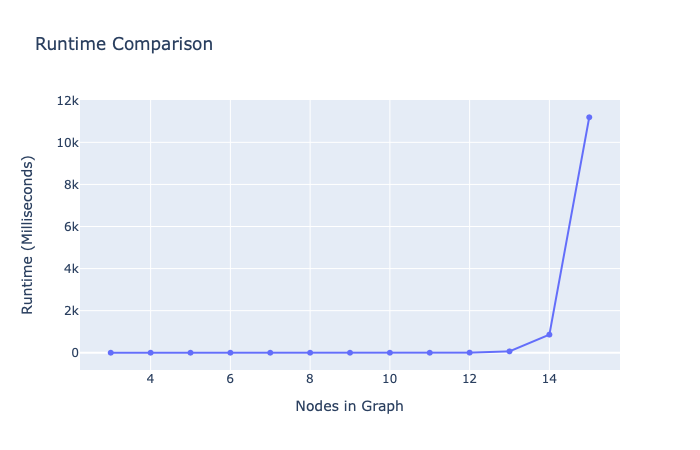
\includegraphics[width=\textwidth]{hk-time.png}
    \caption{Held Karp Execution Time Graph}
    \label{fig:hk-comp}
\end{figure}

The worst case time complexity for this algorithm is the same as the best case since it will always calculate every possible path in order to determine which of them is the shortest. Therefore it has a time complexity of $O(2^n\cdot n^2)$. In order to store the sets of costs, we store all of these possible permutations of paths with a memory complexity of $O(2^n\cdot n)$.

\noindent\textbf{2. Stochastic Local Search:} \texttt{stochastic.js} includes an implementation of the specified random local search algorithm. It can be accessed by including \texttt{const stochastic = require('./stochastic.js');} in the beginning of another node.js file and then calling the function \texttt{stochastic.tsp\_ls} and passing it a valid adjacency matrix. \\

This code was run on the same AWS server as the one used above, and the following data was gathered (Figure 2)\footnote{Data points beyond $n=14$ are excluded to maintain consistency with Figure 1. They continue to increase in accordance with the formula $y=x^3$}.
\begin{figure}[h]
    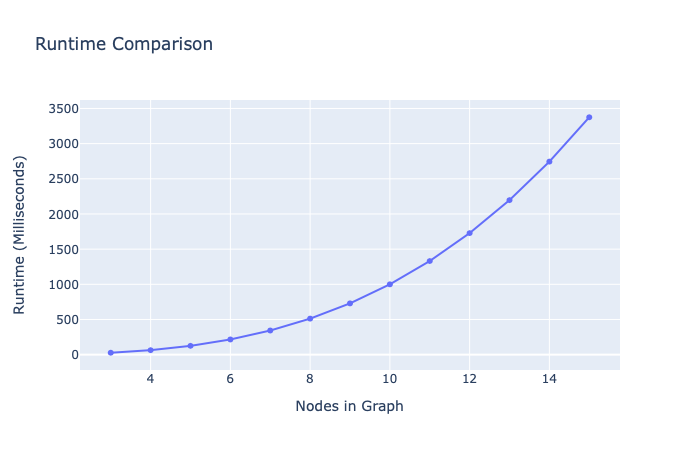
\includegraphics[width=\textwidth]{ls-time.png}
    \caption{Stochastic Local Search Time Graph}
    \label{fig:sl-comp}
\end{figure}

The worst case time complexity for this algorithm is the same as the best case, because it will execute for a set length of time. The purpose of this algorithm is to improve the scalability of the Held-Karp algorithm, so to make it more scalable, it is designed to keep checking randomized paths for $n^3$ seconds, where n is the number of nodes within the graph. The memory for this implementation only stores the adjacency matrix itself and a route, so the worst case memory complexity is $O(n^2 + n)$. \\

\noindent\textbf{3. Comparison} Upon a comparison of the two algorithms, it's clear that depending on the input sizes, either of the two algorithms could be the most useful. For small input sizes, the Held-Karp algorithm is extremely efficient when compared to the two-opt algorithm. Figure 3 shows their relative runtimes plotted on the same graph.
\begin{figure}[h]
    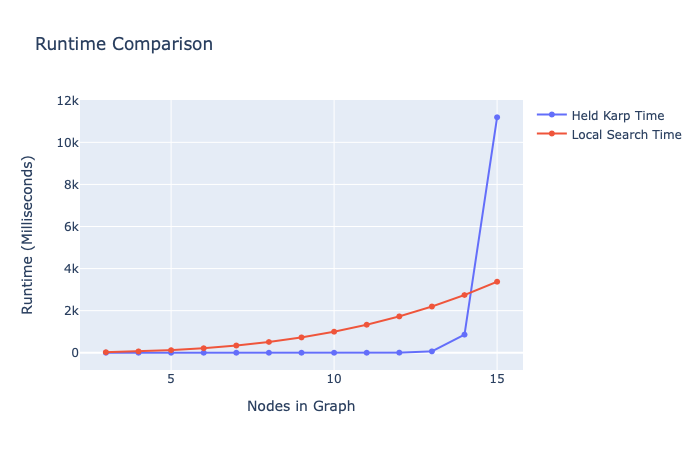
\includegraphics[width=\textwidth]{both-comp.png}
    \caption{Comparison of Empirical Runtime}
    \label{fig:both-comp}
\end{figure}
For further comparison, the differences between their found lowests costs are plotted in Figure 4, and the relative "goodness" of that difference is shown in Figure 5. "Goodness" is a relative term where having a proportionally lower difference is defined a better goodness.
\begin{figure}[tp]
    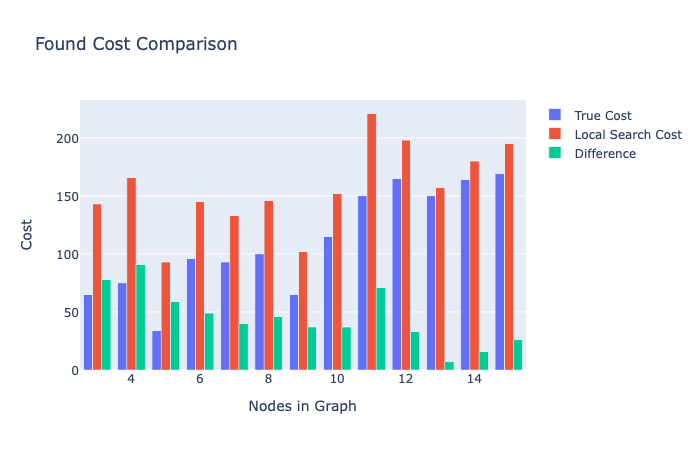
\includegraphics[width=\textwidth]{both-diff.png}
    \caption{Difference in Path Costs}
    \label{fig:both-diff}
\end{figure}
\begin{figure}[bp]
    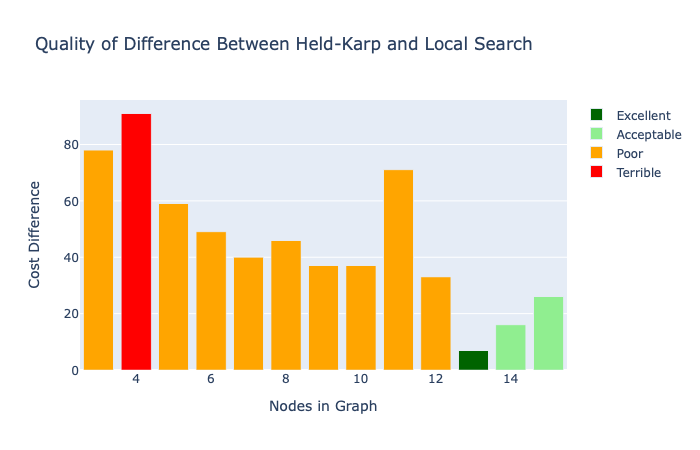
\includegraphics[width=\textwidth]{both-quality.png}
    \caption{Relative Goodness of Difference}
    \label{fig:both-quality}
\end{figure}
In general, it can be seen that over time, the Stochastic Local Search algorithm may be a suitable alternative to the Held-Karp algorithm. While it never found the optimal route in the tests run during this experiment, as the graph size increases, the Local Search cost gets closer to the Held-Karp cost.
\end{document}
